\chapter{Event Selection} \label{chapter:selection}

\section{Introduction}

    Run in parallel with the process of reconstruction is that of event selection.
    As discussed earlier in Chapter \ref{chapter:data},
        there are far too many events in ATLAS to record and analyze them all.
    Thus, a series of selection algorithms are used to veto the abundant background events.
    Unfortunately, these selection algorithms are not perfect,
        and so a careful balance must be achieved between removing a suitable amount of background,
        while retaining as many signal events as possible.

    \begin{figure}[tbh]
        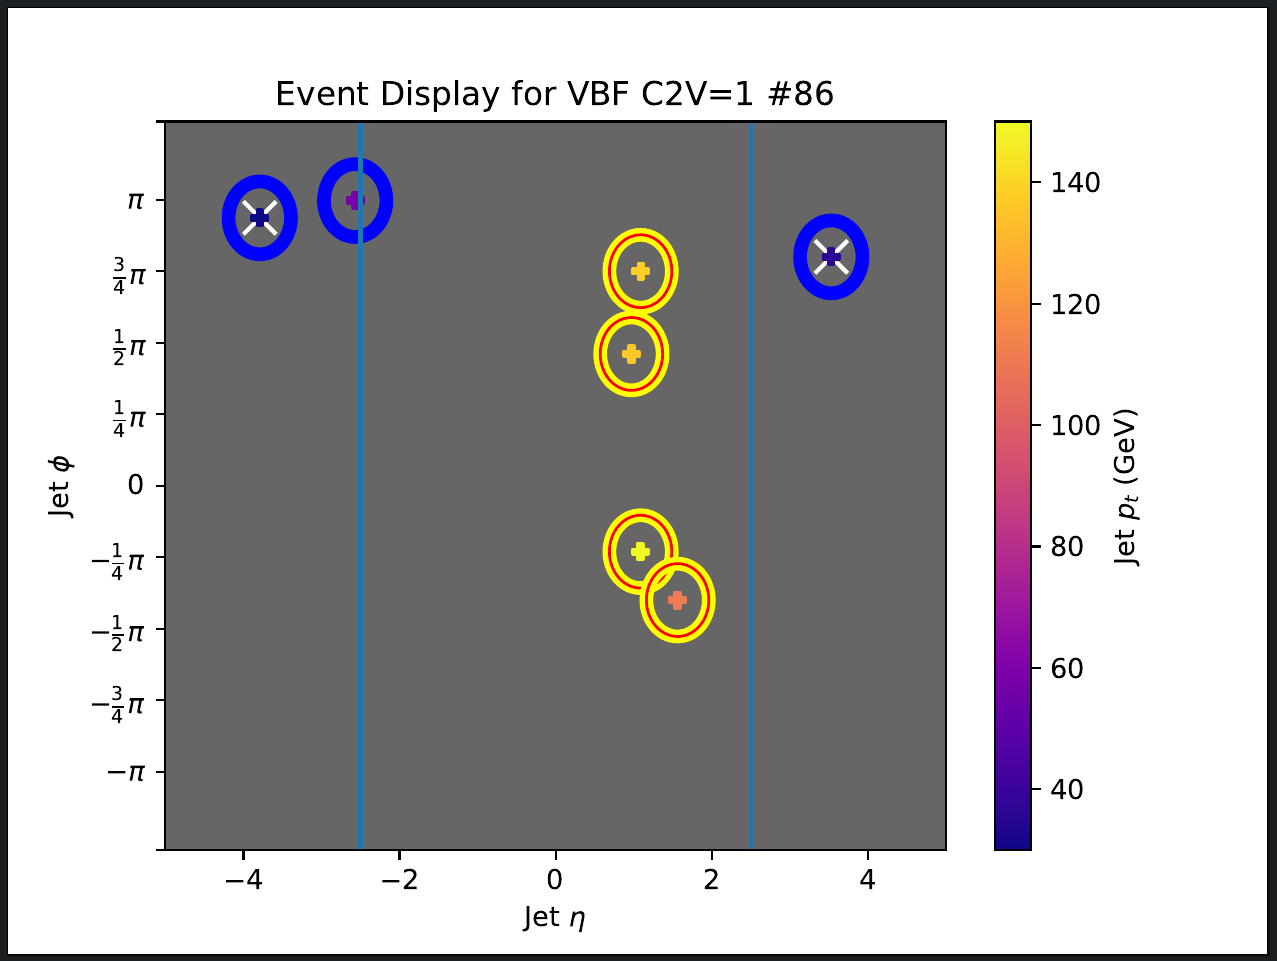
\includegraphics[width=\linewidth,height=\textheight,keepaspectratio]{selection/event_display}
        \caption{
            Event display of a typical \vbfproc event, visualized in $\eta-\phi$ space.
            The various circles correspond to jets in the event.
            The `+' sign in the center of every circle indicates the jet's $p_T$ (scale on right).
            The yellow circles correspond to the b-jet decay products of the Higgs bosons,
                and their red inlay indicates that they have been tagged as b-jets by the b-tagging algorithms.
            The blue jets with white `X's correspond to the VBF initial scatter jets.
            The final blue circle corresponds to a jet caused by a particle radiated by the nearby initial scatter jet.
            The teal vertical lines designate $|\eta|=2.5$,
                the distinction between the ``forward'' and ``central'' regions.
        }
        \label{fig:event_display}
    \end{figure}

    Figure \ref{fig:event_display} is an ``event display'' of what a \vbfhhproc event is expected to look like,
        based on Monte-Carlo simulation (see Chapter \ref{chapter:signal}).
    It demonstrates the key features these selection algorithms use to differentiate signal from background.
    The most obvious feature to identify is the high-$p_T$-jet multiplicity.
    \vbfproc will, by definition, produce a total of six jets;
        the two initial-scatter (IS) light-quark jets, plus the 4 b-jets from the Higgs decay.
    All six of these jets will carry significant energy and transverse momentum.
    A hallmark of the VBF process is the wide opening angle and high invariant mass between the IS jets.
    Such a jet pattern stands out dramatically from most of the stochastic background noise
        and is one of the main advantages of the VBF process.
    Additionally, while the four b-jets of the Higgs are not exclusively produced in the low-$\eta$ regions,
        such a multiplicity of high-$p_T$ b-jets orthogonal to the beamline is rare for background events.
    This makes for another highly identifiable feature of the signal.
    Finally, due to their high initial momentum,
        the $\bbar$ decay products of each Higgs will have only minor angular spread between them,
        producing an identifiable pattern in the final distribution of jets.

    All of these features are exploited by the selection process carried out in this analysis,
        which is performed across two distinct stages.
    The initial selection process is carried out before and during reconstruction, via the aforementioned trigger system.
    After the offline reconstruction process an additional set of selection criteria,
        specific to this analysis, are applied to the fully reconstructed event objects.
    
    \FloatBarrier
    \section{Triggers}
        
        The first stage of the selection process largely occurs before reconstruction has even begun,
            in the L1 and HLT systems as well as Offline reconstruction.
        Table \ref{tab:nr-triggers-used} lists the trigger chains (recall Section \ref{sec:trigger}) used in this analysis.
        An event from ATLAS is incorporated into the data used as long as it passes at least one 
            of the listed chains associated with its year.
        These triggers have been chosen based on any features that lend themselves to the \vbfproc process.
        Notably, the utilized triggers heavily emphasize high jet multiplicity and an abundance of b-jets.
        To understand how, it is necessary to understand the nomenclature of the trigger chains.
        A full reference can be found in Ref. \cite{trigger_naming},
            but a brief example of how to read the chains is provided here:

        HLT\_j110\_gsc150\_boffperf\_split\_2j45\_gsc55\_bmv2c1070\_split\_L1J85\_3J30:
        \begin{itemize}
            \item HLT: These requirements are based in the High Level Trigger
                \begin{itemize}
                \item j110: Requires at least one jet with $E_T$ greater than 110 GeV
                \item gsc150: Requires at least one jet with $p_T \geq 150$ GeV after Global Sequential Calibration (GSC) algorithm is applied
                \item boffperf: The b-jet Offline Performance flavor tagging algorithm has been run on all jets for this event,
                    with its results stored, though no cut is applied at this stage
                \item split: Using ``Split Jets,'' which run the PV algorithms on a superROI
                    that is then split back into individual jet ROIs.
                \item 2j45: Requires at least two jets with $p_T$ of at least 45 GeV
                \item gsc55: Cut on jet $p_T \geq 55$ GeV after jet calibration is applied
                \item bmv2c1070: passes b-jet MV2c10 algorithm at 70\% efficiency level
                \item split: (as above)
            \end{itemize}
            \item L1: These requirements must have been satisfied in the L1 trigger,
                using only the L1 reconstruction (see Section \ref{sec:L1})
                \begin{itemize}
                \item J85: Requires a cluster with energy greater than 85 GeV
                \item 3J30: Require at least 3 jets with a minimum $E_T$ of 30 GeV
            \end{itemize}
        \end{itemize}


        % Triggers used in this analysis and why
        \begin{table}[htbp]
\centering \footnotesize
\begin{tabular}{ccc}
Year                      & Trigger Name                                                                    & \textbf{Trigger Type}  \\ 
\hline
\multirow{2}{*}{2016}                      & HLT\_j100\_2j55\_bmv2c2060\_split                                               & 2b1j                   \\
                      & HLT\_2j35\_bmv2c2060\_split\_2j35\_L14J15.0ETA25                                & 2b2j                   \\

\hline

\multirow{2}{*}{2017}                      & HLT\_j110\_gsc150\_boffperf\_split\_2j35\_gsc55\_bmv2c1070\_split\_L1J85\_3J30  & 2b1j                   \\
                      & HLT\_2j15\_gsc35\_bmv2c1040\_split\_2j15\_gsc35\_boffperf\_split\_L14J15.0ETA25 & 2b2j                   \\

\hline

\multirow{2}{*}{2018}                      & HLT\_j110\_gsc150\_boffperf\_split\_2j45\_gsc55\_bmv2c1070\_split\_L1J85\_3J30  & 2b1j                   \\
                      & HLT\_2j35\_bmv2c1060\_split\_2j35\_L14J15.0ETA25                                & 2b2j                   \\
                
\end{tabular}
\caption{Triggers used for non-resonant searches.\cite{hh4b_2021_int_note}}
\label{tab:nr-triggers-used}
\end{table}

        % (do we have any plots showing why we use these triggers?)
        %   Yes, though I might be able to get away without using them

        %Trigger bucketing strategy? What are the chances I can just not deal with this?


\FloatBarrier
\section{Analysis Cuts} \label{sec:analysis_cuts}

        Upon completion of the ATLAS-wide trigger selection,
            the appropriate data samples are copied for use by this analysis.
        However, the available data still contain a vast excess of background events
            consisting of QCD multijet, \ttbar, gluon-gluon fusion (ggf), and single Higgs process events.
        A ZZ \to 4b process was also considered as a potential background.
        MC simulation shows that the ZZ production is highly forward and low-$p_T$,
            resulting in very low acceptance through the selection criteria described below
            and thus negligible as a background \cite{vbf_hh_4b_resonant_2020_int}.
        Similarly, the yield and acceptance of the ggf and single Higgs processes, though substantial,
            were found through MC simulation to be dwarfed by the QCD multijet background\cite{hh4b_2021_int_note}.
        The only backgrounds that are therefore considered for this analysis are the
            dominant QCD multijet background and sub-dominant \ttbar background.

        To mitigate the effects from these backgrounds,
            this analysis makes an additional series of selection cuts on the fully reconstructed events.
        These cuts focus on the topological features discussed earlier,
            selecting events based on their jet multiplicity,
            the VBF jet kinematics,
            and the angular clustering of the Higgs decay products.

    \FloatBarrier
    \subsection{Jet Multiplicity and Categorization}
        
        First and foremost is a check to ensure that there are enough jets to even constitute a \vbfproc event,
            by emphasizing the quality and location of jets.
        Jets are categorized as ``central'' if they fall within $|\eta| \leq 2.5$
            and are ``forward'' if they are found with $ 2.5 < |\eta| \leq 4.5 $.
        The reason for the distinction between the two is that central jets fall within the boundaries of the ATLAS tracker system
            (see Section \ref{sec:inner_detector}).
        As the tracking system is necessary for the b-tagging algorithms,
            candidates for the Higgs' decay products are taken exclusively from central jets.
        To suppress jets from pileup vertices, central jets are only used if they have a $p_T > 40$ GeV,
            and satisfy at least one of the following three conditions:
            they pass the JVT algorithm\footnote{
                The Jet-Vertex-Tagger (JVT) algorithm is a pileup vertex suppression discriminant,
                    derived from the $p_T$ of the jets and its constituent tracks\cite{jvt_algo}.
            }, have $p_T > 60$ GeV, or have $2.4 < |\eta| < 2.5$.
        Forward jets have less stringent requirements, needing only a $p_T > 30$ GeV.

        After jets have been categorized and selected, an event is only used if there are at least six selected jets remaining.
        Of these, at least four must be central jets which have been b-tagged by the offline DL1r algorithm at the 77\% working point.
        From the remaining jets (central or forward), there must be at least two \textit{anti}-b-tagged jets
            (i.e.\ jets that were marked as failing the b-tagging requirement).

        The VBF jets are chosen as the pair of anti-b-tagged jets with the largest vector-sum invariant mass (\mjj) between them,
            while the Higgs decay jets are chosen as the four highest-$p_T$, b-tagged, central jets.
        Any other jets in the event are discarded for the purposes of the rest of the analysis.
        The remaining selection cuts are made on these two categories of jets.
        

    \subsection{VBF Topology}

        For the VBF jets, the characteristic wide-opening angle and high invariant mass is exploited here.
        The selected VBF pair must have $\deta > 3$ and $\mjj \geq 1000 \textrm{GeV}$.
        As well, the combined vector-sum-$p_T$ of all six jets
            (the four Higgs products and the two VBF jets)
            must be less than 65 GeV:
        \begin{equation}
            \vec{p}_{\textrm{sum}, p_T} \leq 65 \textrm{GeV} \quad;\quad
            \vec{p}_{\textrm{sum}} \equiv
            \vec{p}_{b1} + \vec{p}_{b2} + 
            \vec{p}_{b3} + \vec{p}_{b4} +
            \vec{p}_{j1} + \vec{p}_{j2} 
            \,.
        \end{equation}
        The maximum sum-$p_T$ requirement follows from the fact that the initial incoming beamline particles have
            very low transverse momentum\footnote{
                Initial state radiation can cause the VBF+4b system to have some tranverse momentum,
                    hence the upper-bound on this cut.
            }, and so the output of their interaction should as well.
        These specific values for the cuts are based on the significance values
            (defined as the ratio of the number of signal events to the square root of the number of background events)
            shown in Fig. \ref{fig:vbf_cuts}.

        \begin{figure}[tbh]
            \begin{subfigure}{0.48\textwidth}
                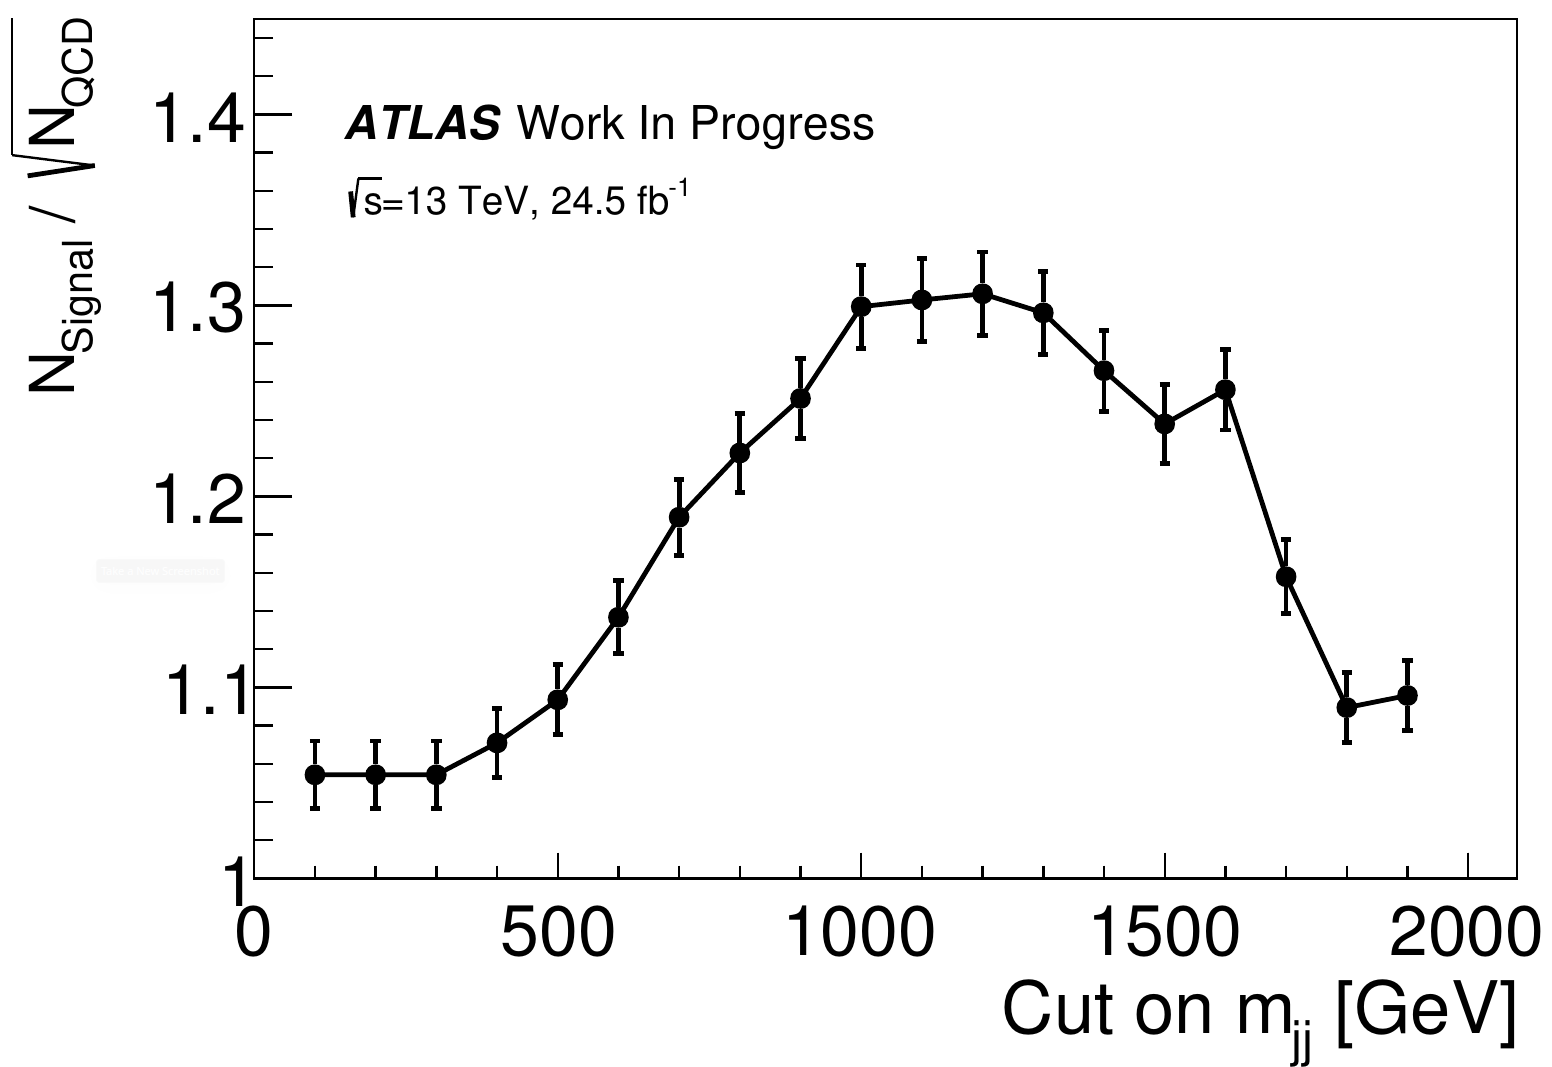
\includegraphics[width=\linewidth,height=\textheight,keepaspectratio]{selection/mjj_significance}
                \caption{$m_{jj}$ Cut Significance}
            \end{subfigure}
            \begin{subfigure}{0.48\textwidth}
                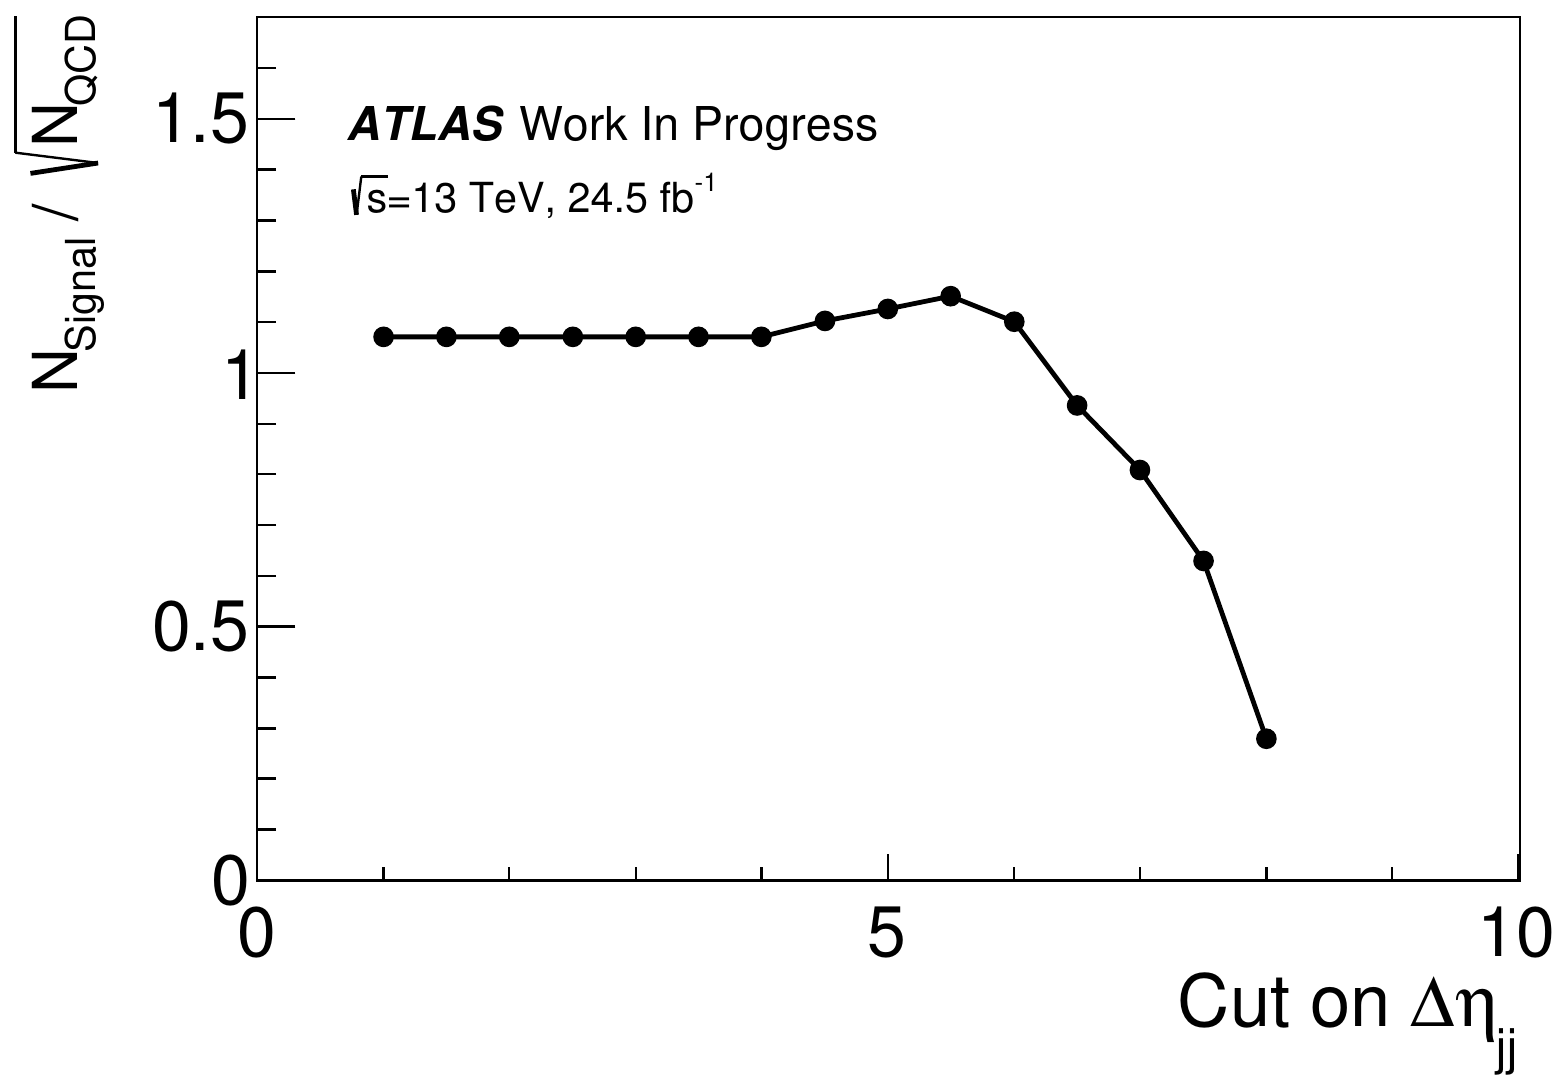
\includegraphics[width=\linewidth,height=\textheight,keepaspectratio]{selection/detajj_significance}
                \caption{$\deta_{jj}$ Cut Significance}
            \end{subfigure}\\
            \begin{subfigure}{0.48\textwidth}
                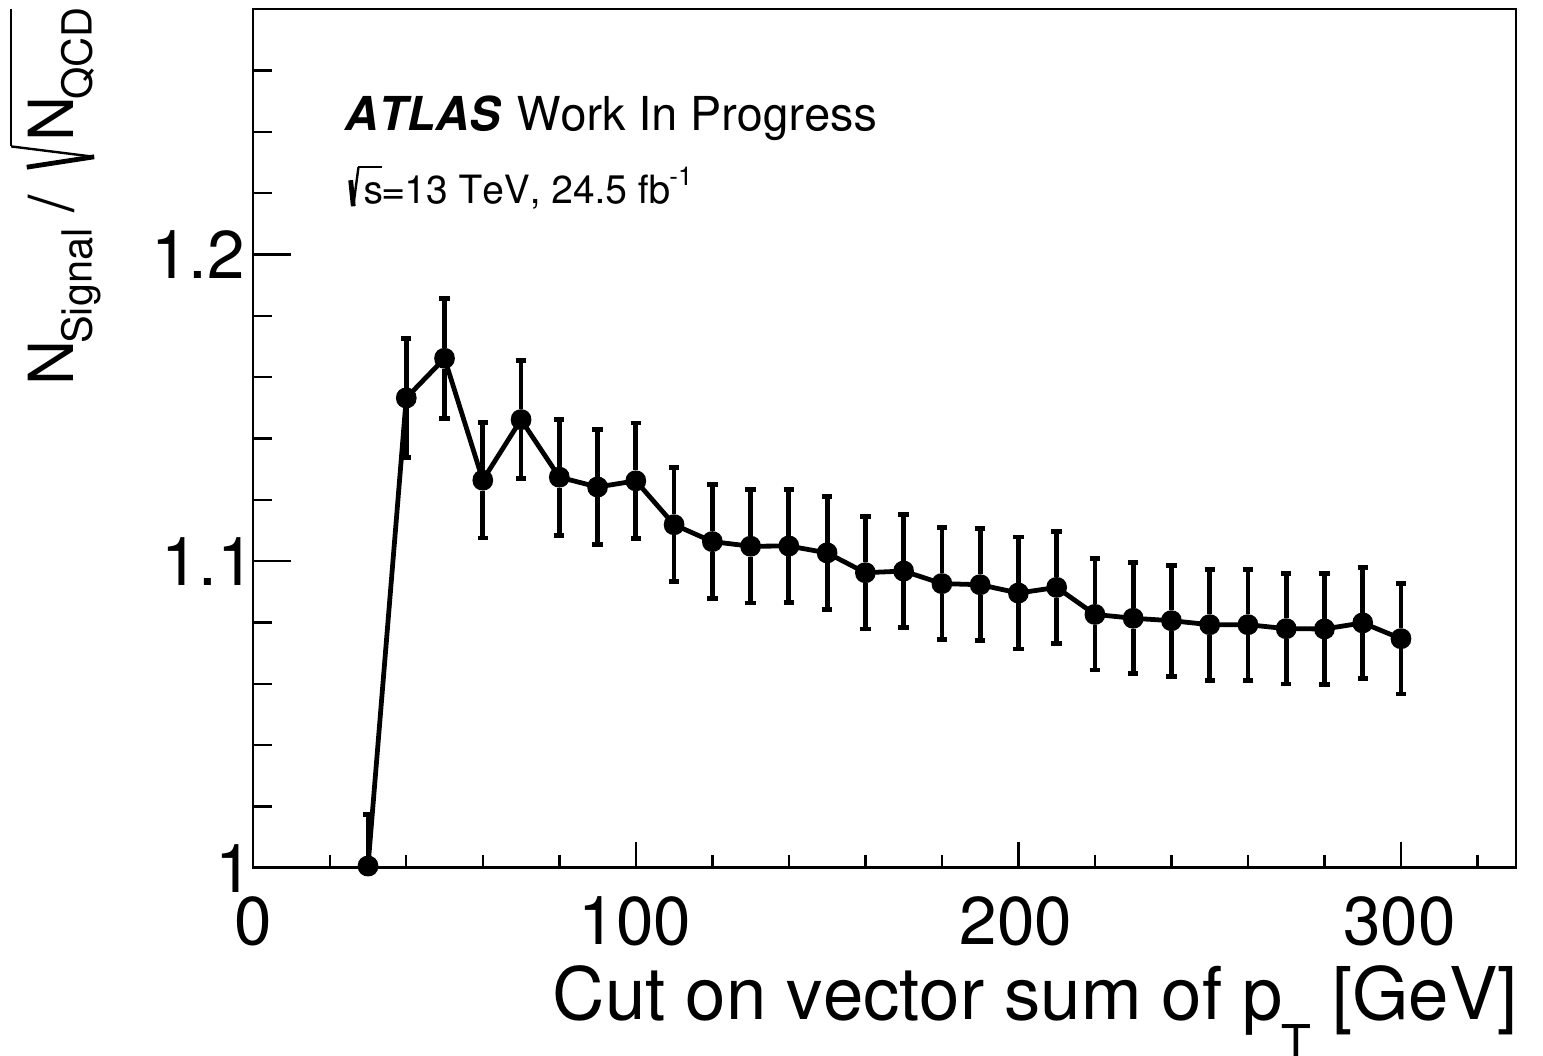
\includegraphics[width=\linewidth,height=\textheight,keepaspectratio]{selection/vecsum_pt}
                \caption{6-Jet Vector-Sum $p_{T}$ Cut Significance}
            \end{subfigure}
            \caption{
                Significance value for different cut values on the various VBF selection criteria\cite{vbf_hh_4b_2018_int}.
                Specifically, cuts on \mjj and $\Delta \eta_{jj}$ denote the \textit{minimum} value permitted,
                    while the cut on ``vector sum of $p_T$'' is an upper bound.
                The goal is to maximize significance while avoiding ``edges'' where significance rapidly falls off.
                The selection cuts chosen for this analysis can be seen to occupy roughly the middle
                    of the highest points of these plots.
                For example, the peak at $\Delta \eta_{jj} = 5$ is avoided due to its proximity
                    to the sudden drop in significance immediately to its right.
            }
            \label{fig:vbf_cuts}
        \end{figure}


    %\FloatBarrier
    \subsection{B-Quark Pairing}

        What is detected within ATLAS and reconstructed by Athena are not Higgs Bosons, but rather their decay products.
        To reconstruct the two Higgs Bosons, the four reconstructed b-quarks must be combined together, two b's to each Higgs.
        A pairing algorithm called MinDR\cite{hh4b_2021_int_note}
            is used to determine the optimal pairing.
        MinDR operates under the assumption that the decay products of the Higgs boson
            should be relatively close to each other in angular space, consistent with the Higgs's high $p_T$.
        With four jets, which need to be split into two pairs, there are three ways to choose the pairings.
        For each of the three unique pairing options, MinDR takes the pair with the leading $p_T$ as the ``leading Higgs Candidate.''
        The pairing option that minimizes the $\Delta R$ between the leading Higgs Candidate decay products
            (see Fig. \ref{fig:minDR_pairing_diagram}) is chosen.
        The effectiveness of this algorithm has been validated for multiple values of \kvv and \kl,
            as shown in Fig. \ref{fig:HHpairing}.

        \begin{figure}[tbh]
            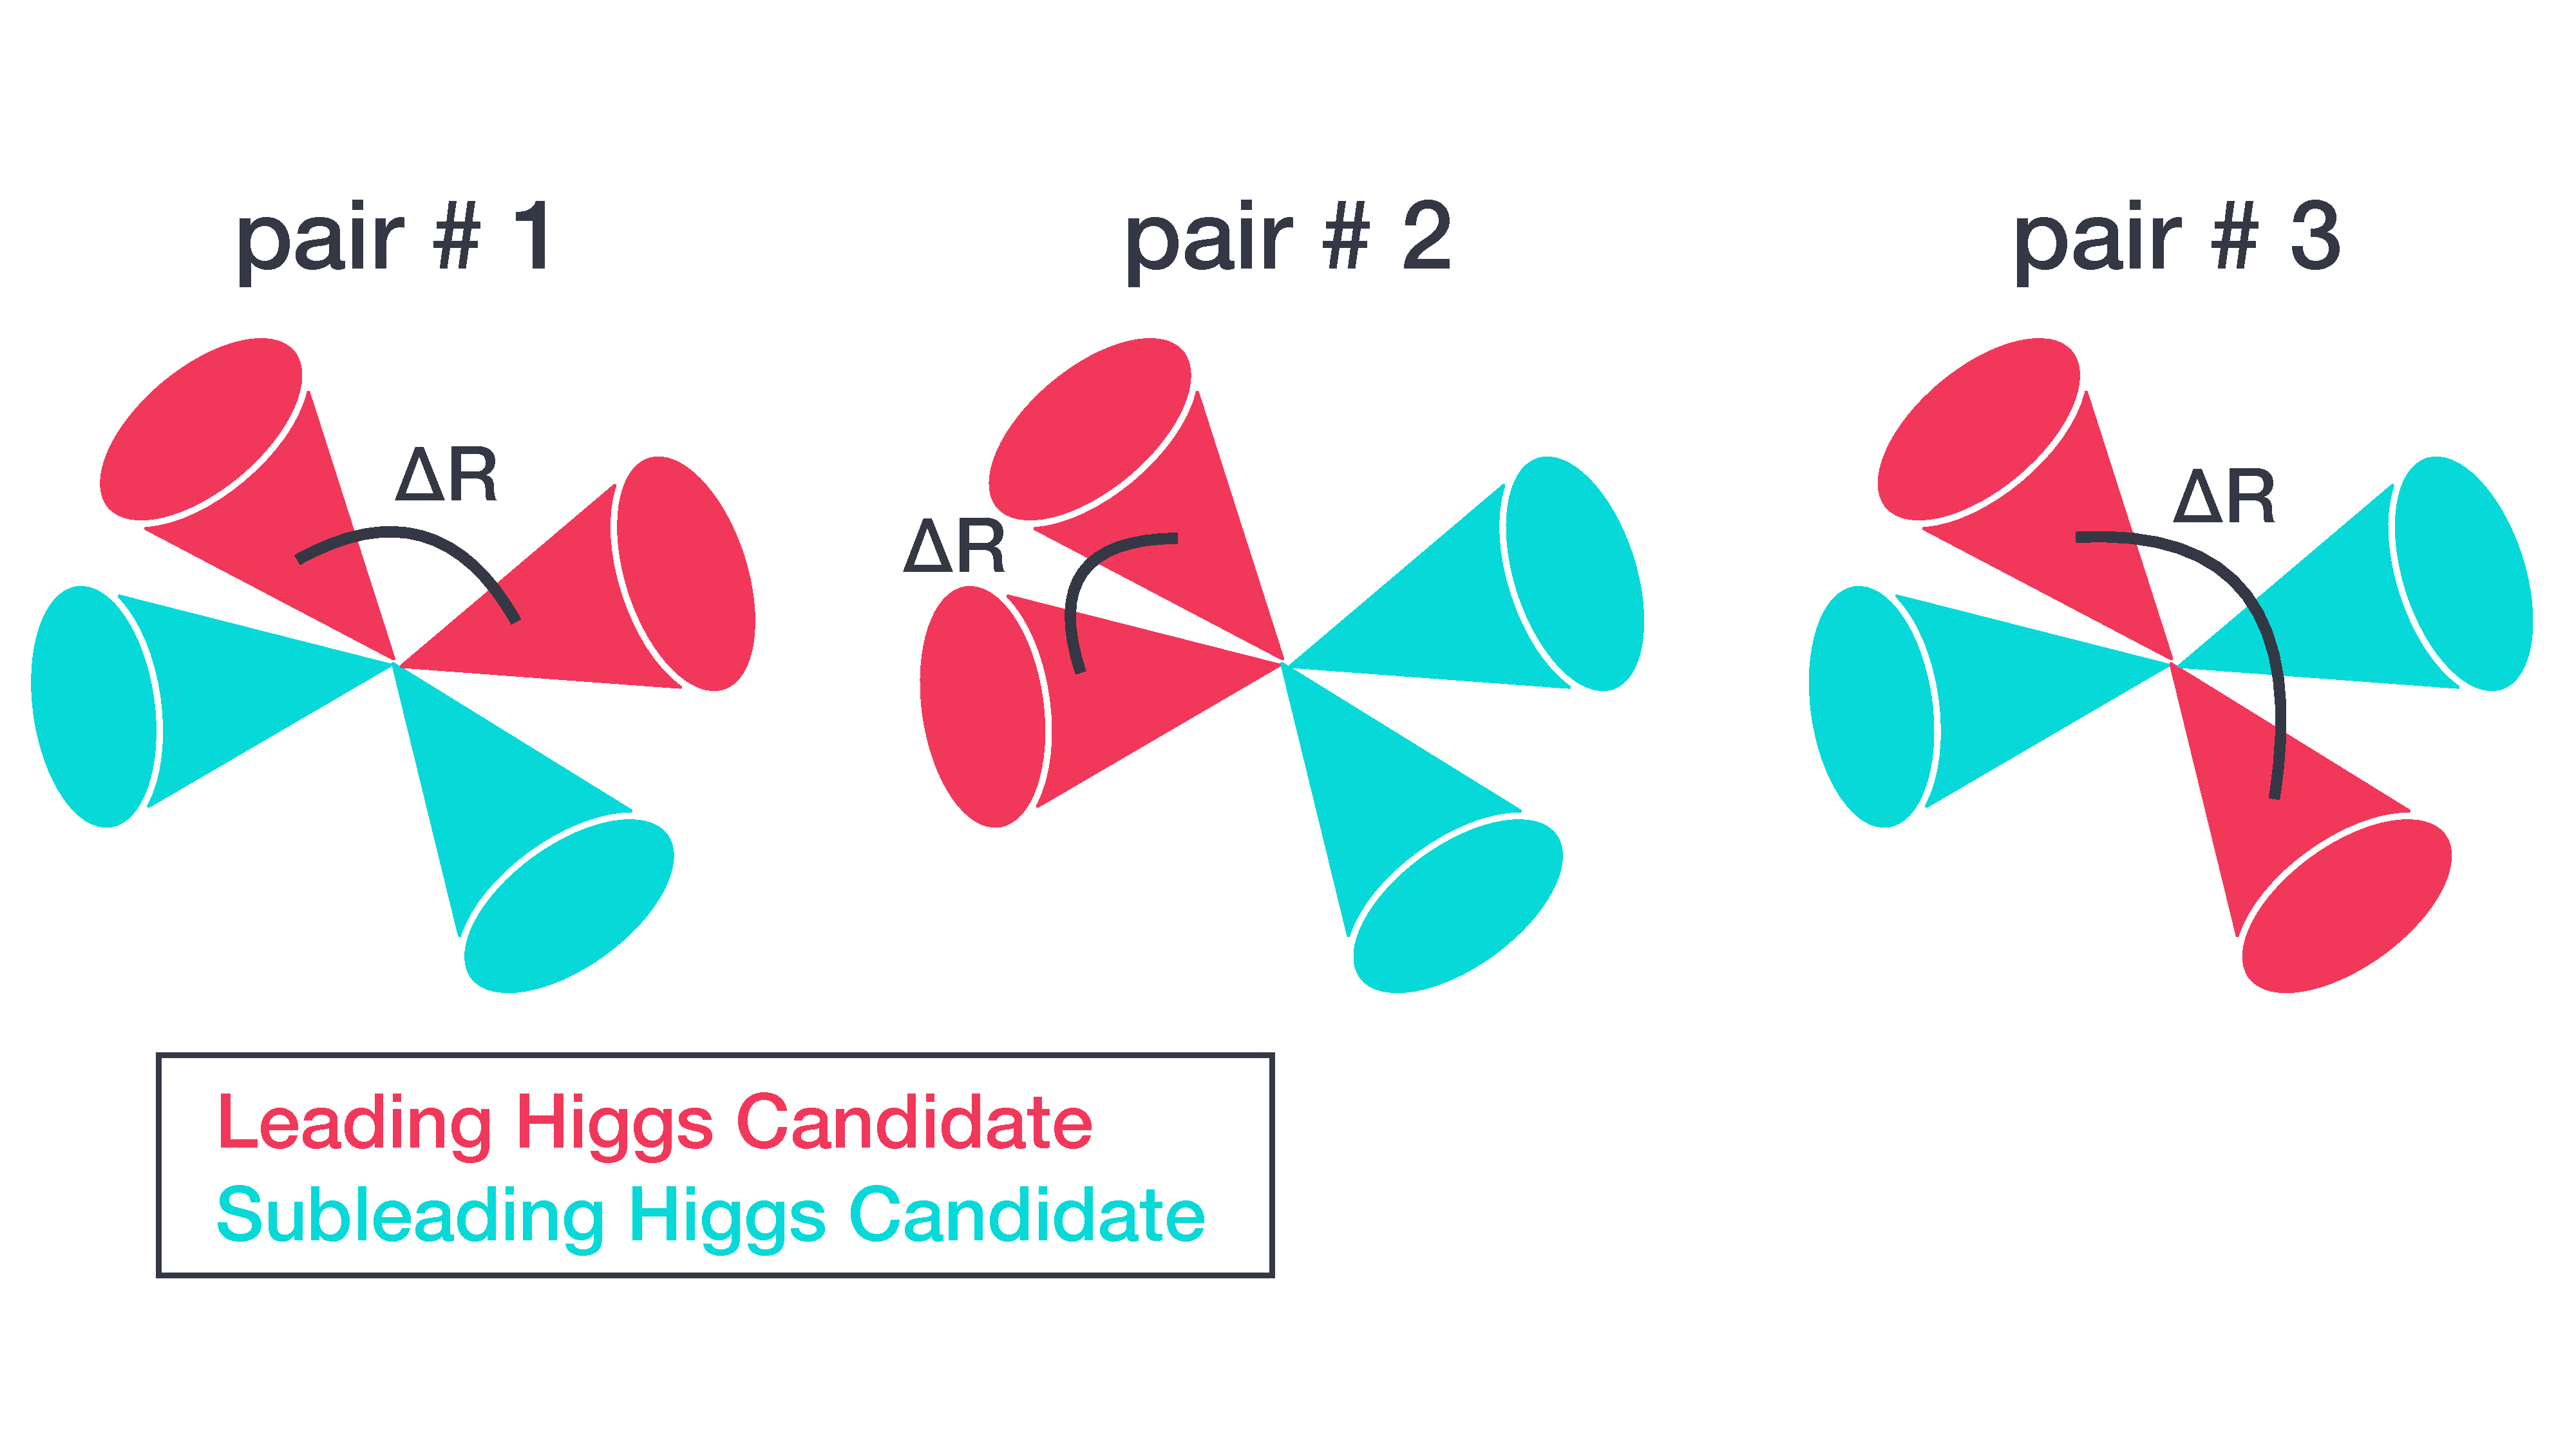
\includegraphics[width=\linewidth,height=\textheight,keepaspectratio]{selection/pairing}
            \caption{
                A diagram showing how the MinDR algorithm functions.
                For the 4 b-jets, there are three unique pairings.
                For each pair, the candidate Higgs boson is reconstructed and its $p_T$ recorded.
                The reconstructed Higgs with the highest $p_T$ of the two is the labeled the Leading Candidate
                    (the red jets).
                MinDR will selected the pairing which reduces the $\Delta R$ between the constituent jets
                    of the leading Higgs candidate pair (which in this example would be pair \#2)\cite{hh4b_2021_int_note}.
            }
            \label{fig:minDR_pairing_diagram}
        \end{figure}


        \begin{figure}[hbt]
            \centering
            \begin{subfigure}{0.48\textwidth}
                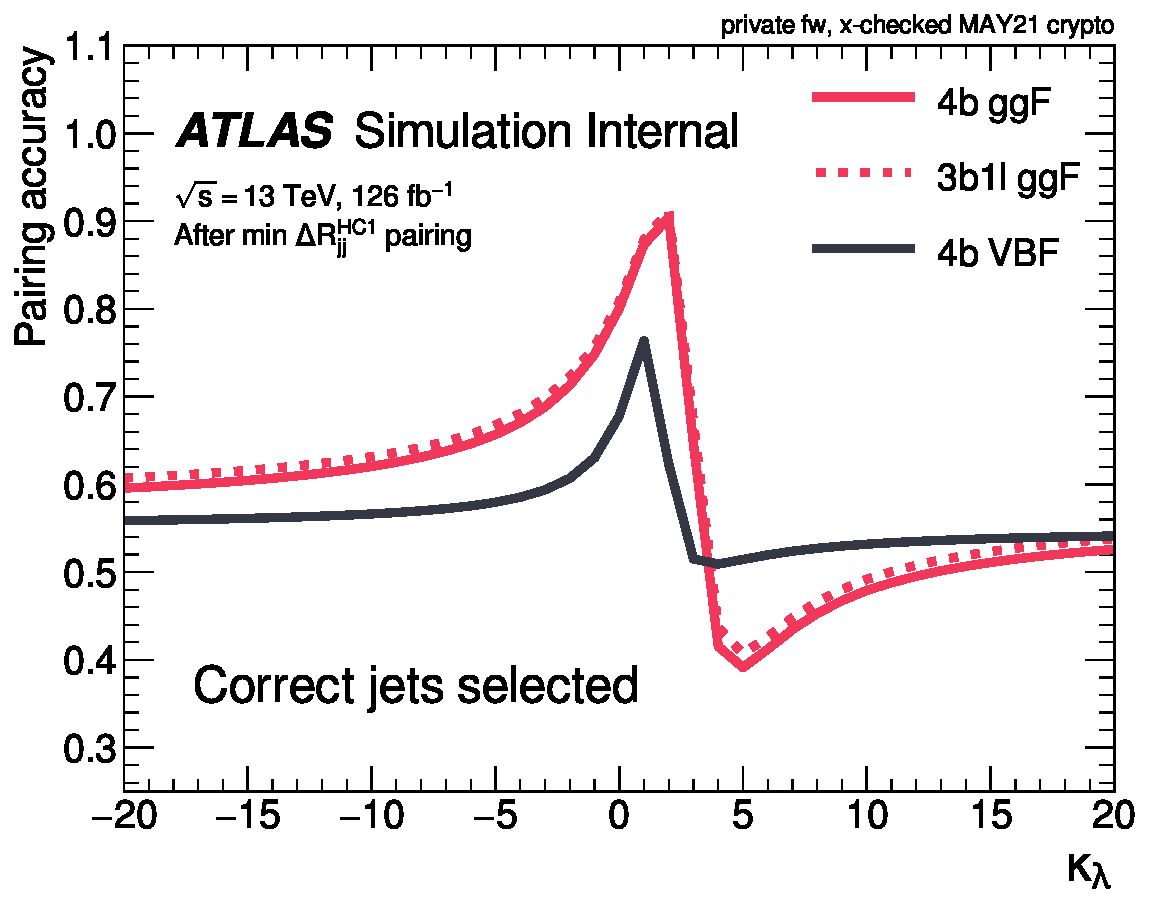
\includegraphics[width=\textwidth]{selection/pairing_accuracy_kl}
                \captionsetup{justification=centering} \caption{Pairing accuracy vs \kl}
                \label{fig:acc_kl_exists}
            \end{subfigure}
            \begin{subfigure}{0.48\textwidth}
                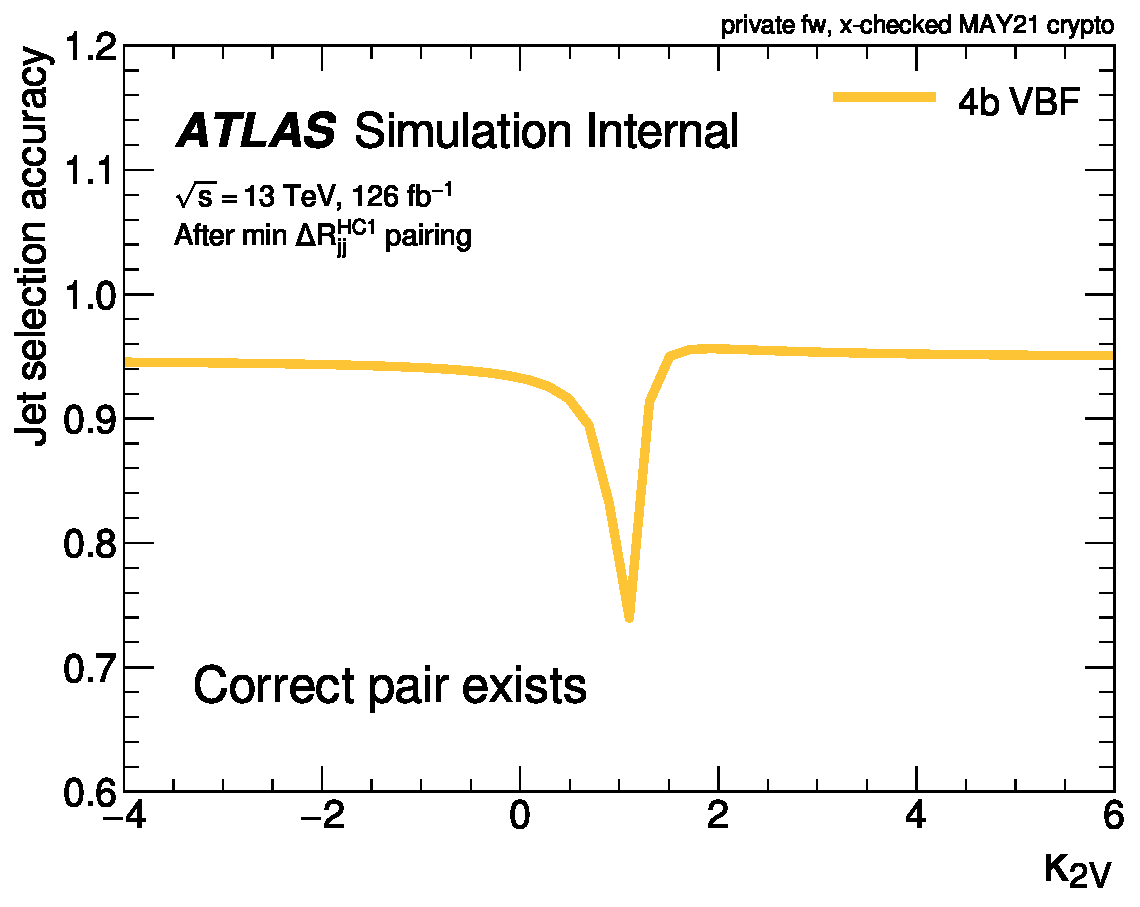
\includegraphics[width=\textwidth]{selection/pairing_accuracy_k2v}
                \captionsetup{justification=centering} \caption{Pairing accuracy vs $\kappa_{2V}$}
                \label{fig:acc_k2v_exists}
            \end{subfigure}
            \caption{Accuracy of the MinDR pairing algorithm for different values of \kv and \kvv.
                Accuracy here is defined as the fraction of events which were paired correctly,
                compared to all events in which the correct 4 Higgs decay b-jets were given to the algorithm.
                Worst case accuracy (random guessing) would produce 33\% accuracy,
                    so even at the algorithm's worst (~50\%),
                    it still performs much better than random association.
                The algorithm has its lowest performance for $\kl \approx 2$ and $\kvv \approx 1$,
                    for which the produced Higgs bosons are the softest.
                For variations of the couplings (especially \kvv),
                    the pairing accuracy is far better at 95\% \cite{hh4b_2021_int_note}.
                %If needed, Figure 19 of the note also gives this as a function of mhh
                }
            \label{fig:HHpairing}
        \end{figure}
                                                                                                         


    \FloatBarrier
    \subsection{ Region Definition and \ttbar Removal}
        
        There are three ``regions'' that are used for the analysis.
        Control Region 1 and 2 (CR1 and CR2) are used for the Background Estimation (see Chapter \ref{chapter:background}).
        The ``Signal'' Region is the set of data which will be used to search for the di-Higgs process.

        Which region an event falls into is based on the reconstructed masses of the leading and sub-leading Higgs.
        The Signal Region (SR) corresponds to those events for which the reconstructed Higgs masses
            align closely with the measured value of the Higgs Boson (125 GeV),
            with additional room provided for error in the mass measurement.
        CR1 and 2 are adjacent to the SR, designating events with kinematics very similar to the Signal Region,
            but with reconstructed Higgs masses incompatible with experimental measurement (see Fig. \ref{fig:region_definition}).
        A quantity $X_{HH}$ governs the boundaries of these regions,
            which effectively acts as a $\chi^2$ fit on the expected Higgs masses,
            and is defined as
        \begin{equation} \label{eq:xhh}
            X_{HH} \equiv \sqrt{\left(\frac{m_{H1} - 124\textrm{GeV}}{0.1 \ m_{H1}}\right)^{2}
                + \left(\frac{m_{H2} - 117\textrm{GeV}}{0.1 \ m_{H2}}\right)^{2}}
            \,.
        \end{equation}

        The \mhh parameters 124 and 117 were chosen to match the center of the \mhh distributions
            of the leading and sub-leading reconstructed Higgs bosons for
            MC simulations of the $\kvv = 0$ signal variation
            (note the position of the center of Fig. \ref{fig:region_definition}).
        $X_{hh} < 1.6$ defines the SR,
            while CR1 and CR2 are set within a ring-like shape between the SR
            and an outer boundary defined by
        \begin{equation} \label{eq:cr_out}
            \text{CR\ Outer\ Edge} \quad : \quad \sqrt{ \left(m_{H1} - 1.05 \cdot 124\textrm{GeV}\right)^2
                +  \left(m_{H2} - 1.05 \cdot 117\textrm{GeV}\right)^2 } = 45\textrm{GeV}
            \,.
        \end{equation}
        
        CR1 and CR2 are divided based on studies demonstrating that this choice results in
            close kinematic similarity between the two regions.

        \begin{figure}[tbh]
            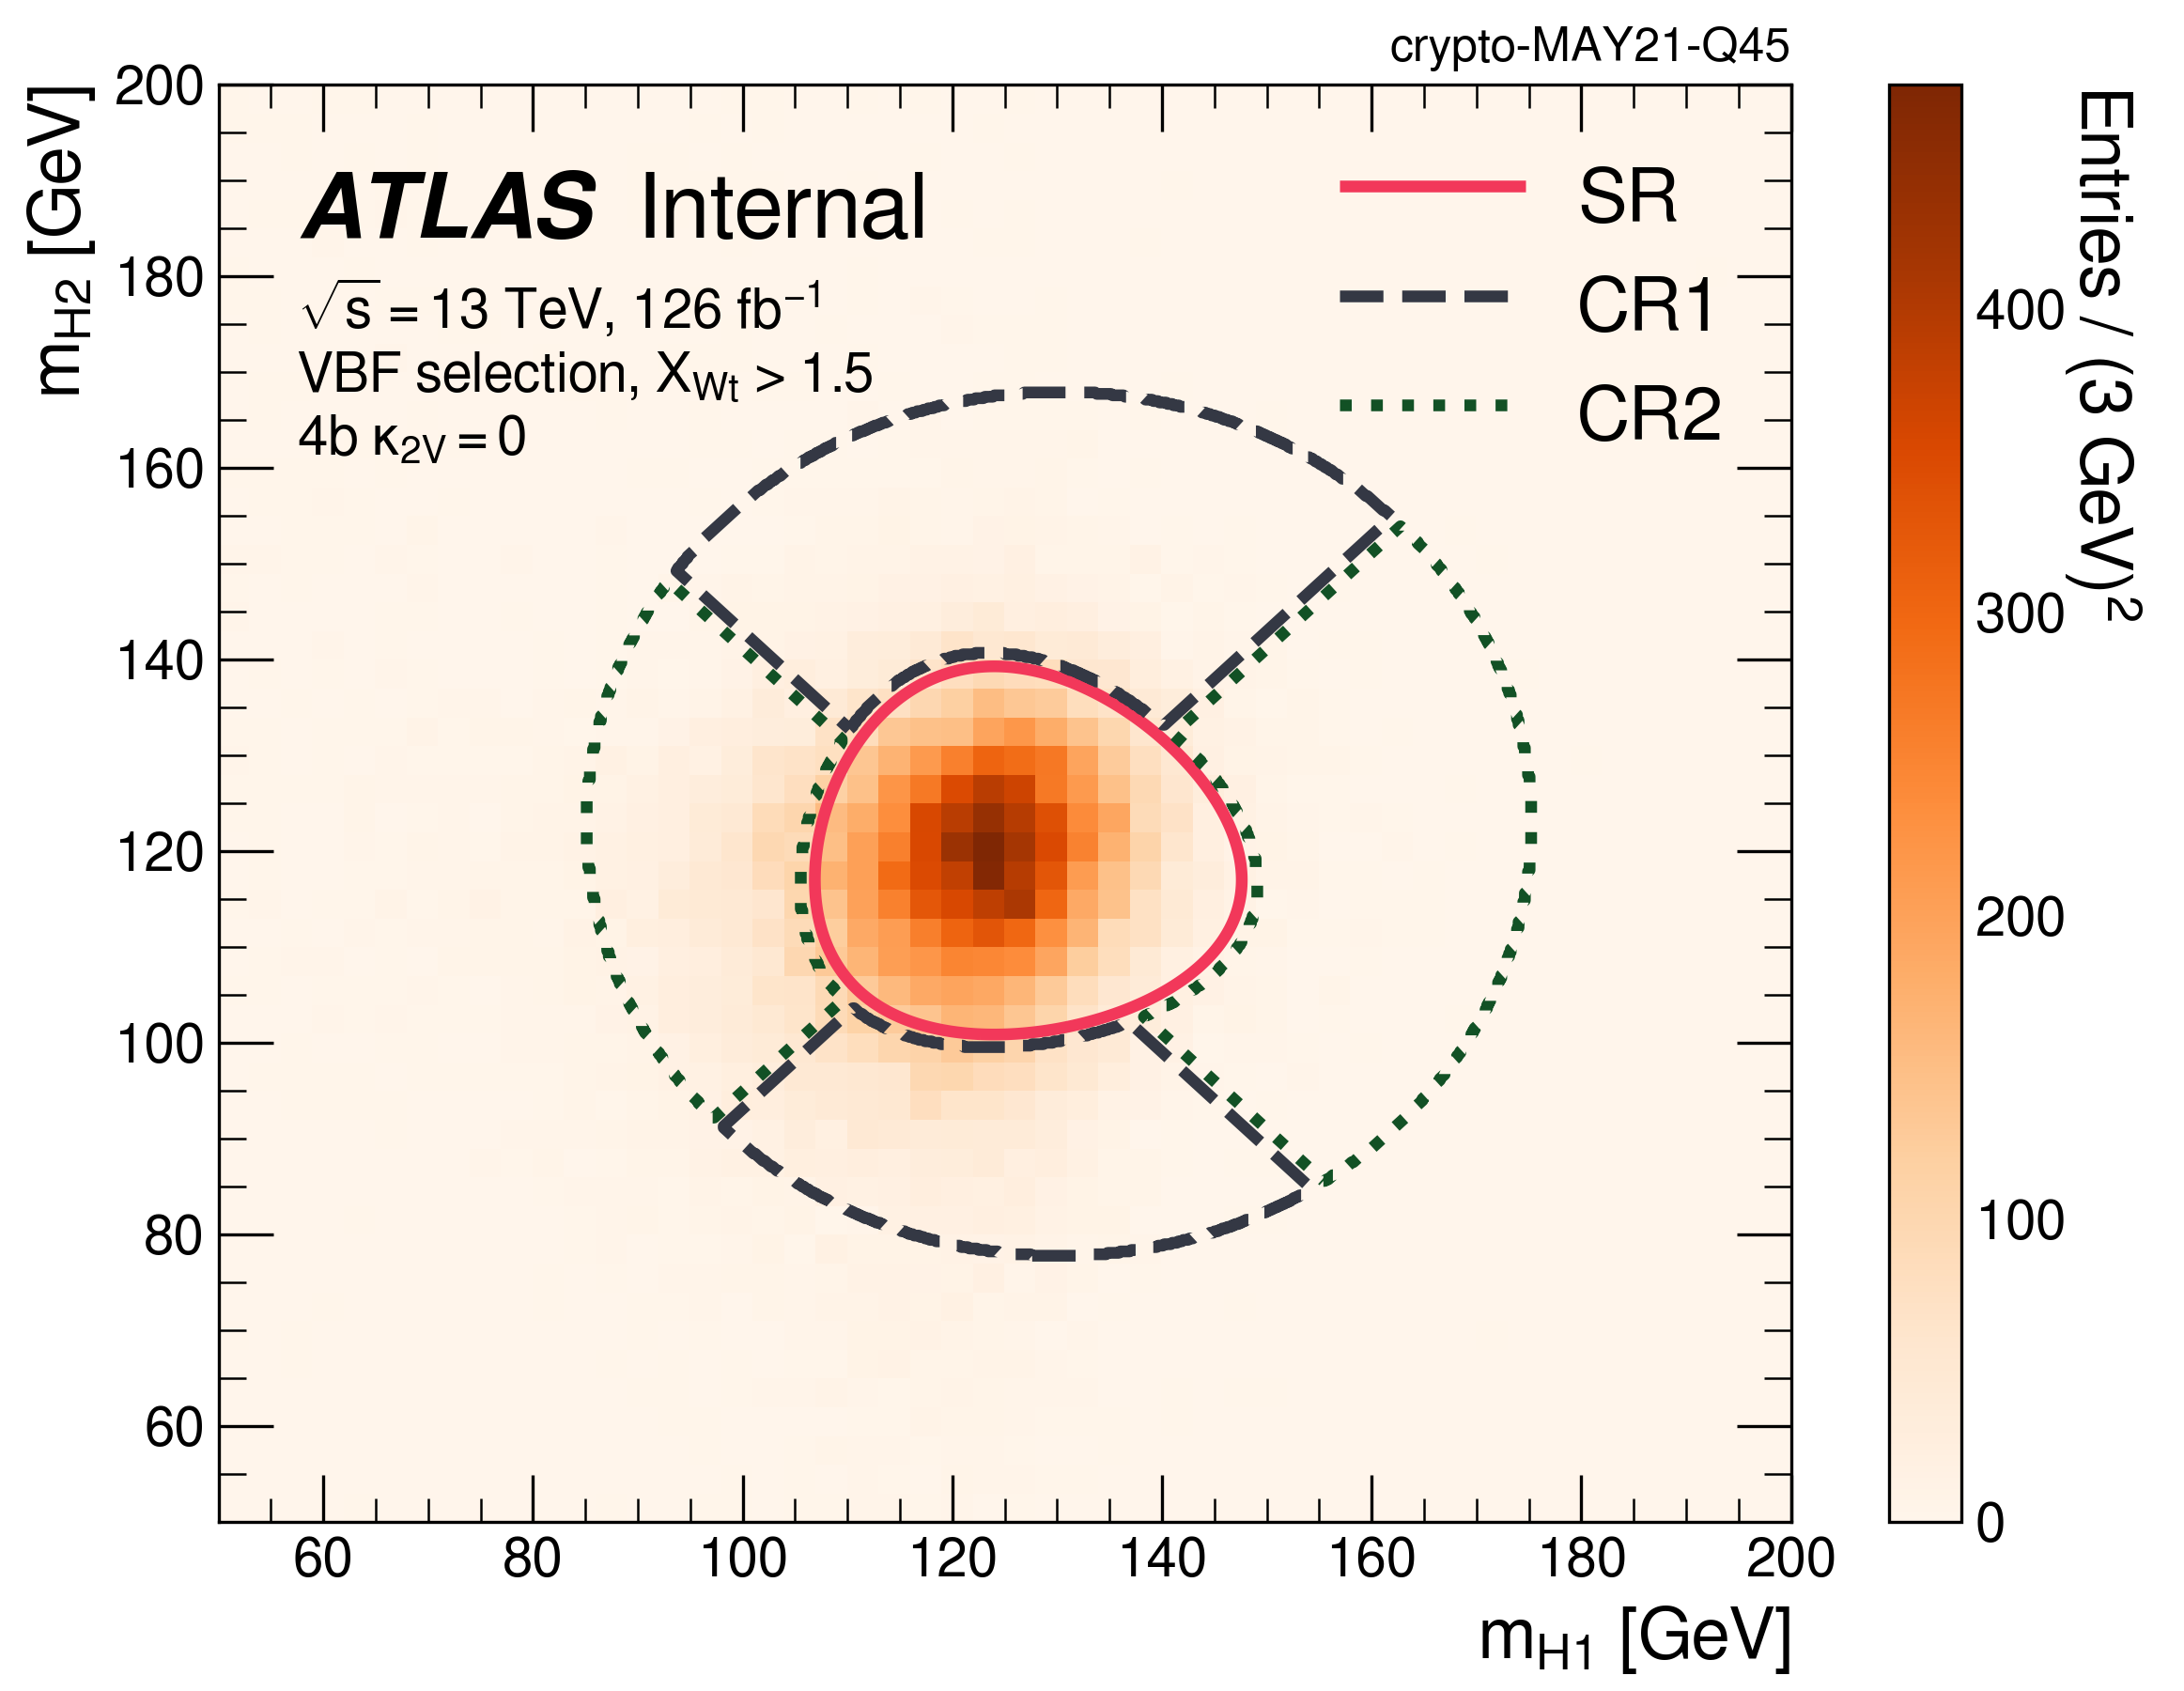
\includegraphics[width=\linewidth,height=\textheight,keepaspectratio]{selection/massplane_sig_all_4b_vbf_Xwt_1p5_k2V_0}
            \caption{
                A 2D histogram of MC signal events (\kvv=0), showing how the analysis regions are defined.
                The SR is centered on the peak of the 2D distribution and extends out to encompass nearly all events.
                The Control Regions are defined within a ring around the SR,
                    with CR1 and 2 split across four quadrants.
                CR1 is split between the top and bottom quadrants,
                    while CR2 occupies the left and right quadrants.
                \cite{hh4b_2021_int_note}
            }
            \label{fig:region_definition}
        \end{figure}

        \FloatBarrier
        Following the region definition the one step of selection remaining is the Top veto cut, \xwt.
        \xwt is a discriminating variable constructed in a similar manner to $X_{hh}$,
            but for the purpose of reducing the \ttbar background.
        It is produced first by taking all possible pairs of jets with $p_T > 40$ GeV and $|\eta| < 2.5$
            (regardless of whether they were matched to VBF jets, or b-jets, or neither),
            and reconstructing a W-boson from that pair.
        Top quark candidates are formed from any remaining b-jets that were used as Higgs candidates.
        There are many W-boson candidates, and many Top quark candidates for each possible reconstructed W-boson.
        For each combination, the reconstructed masses of the W-boson $m_W$ and Top quark $m_t$
            are used as inputs for the formula
        \begin{equation} \label{eq:xwt}
            \xwt \equiv \sqrt{\left(\frac{m_W - 80.4\textrm{GeV}}{0.1 \ m_W}\right)^{2}
                + \left(\frac{m_t - 172.5\textrm{GeV}}{0.1 \ m_t}\right)^{2}}
            \,.
        \end{equation}

        If any of the pairs is found to have an \xwt value less than 1.5, the event is vetoed. 
        \ttbar MC has been used to measure the effectiveness of the \xwt cut,
            and has been found to reduce the yield of this process from
            12.2\% of the total background contribution to only 8.1\%.
        Of course, a large number of \ttbar events still remain,
            as does the much larger contribution from QCD multijet events.
        The contribution of these remaining background events to the total signal yield
            must now be estimated.
        To do this, the analysis employs a data-driven approach.


        \begin{figure}[tbh]
            \begin{subfigure}{0.48\textwidth}
                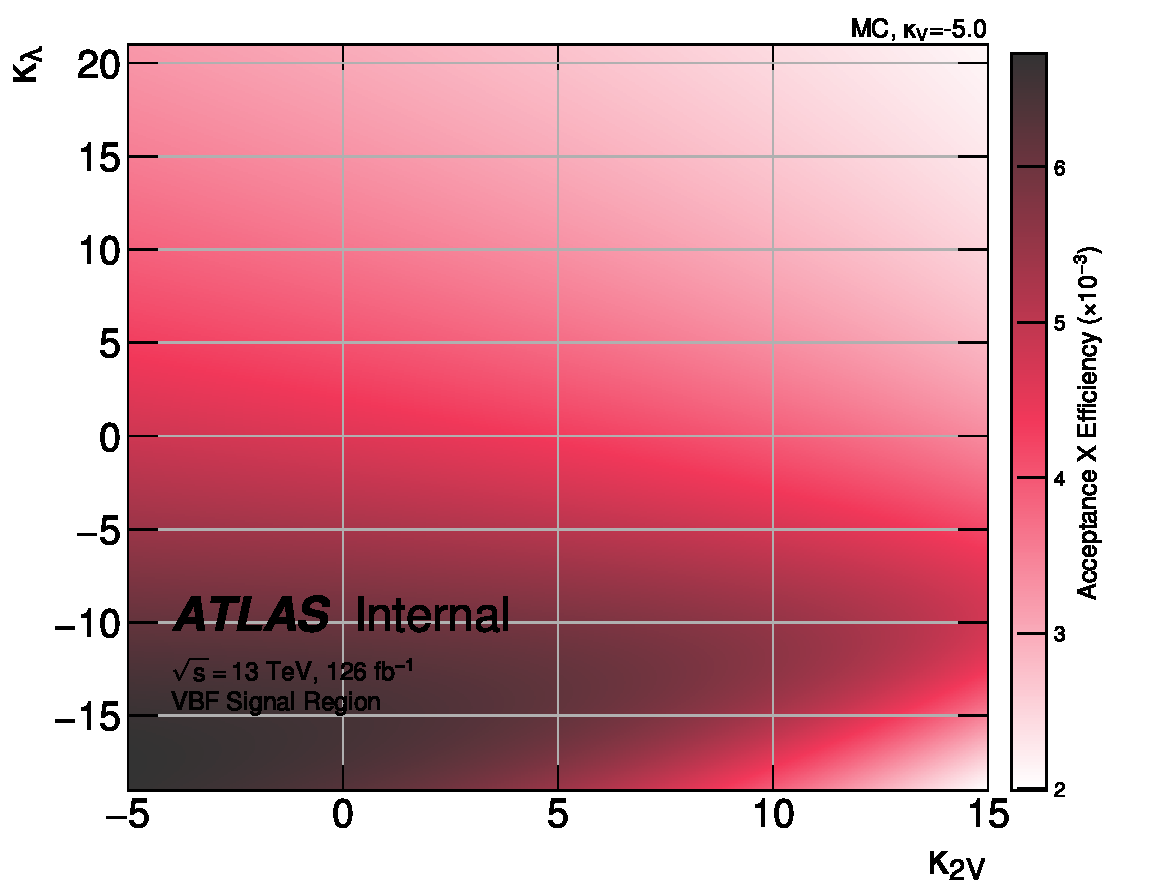
\includegraphics[width=\linewidth,height=\textheight,keepaspectratio]{selection/VBF2D-vbf-MC-Signal-Region-all-4b-accXeff-kv-5p0}
                \caption{}
            \end{subfigure}
            \begin{subfigure}{0.48\textwidth}
                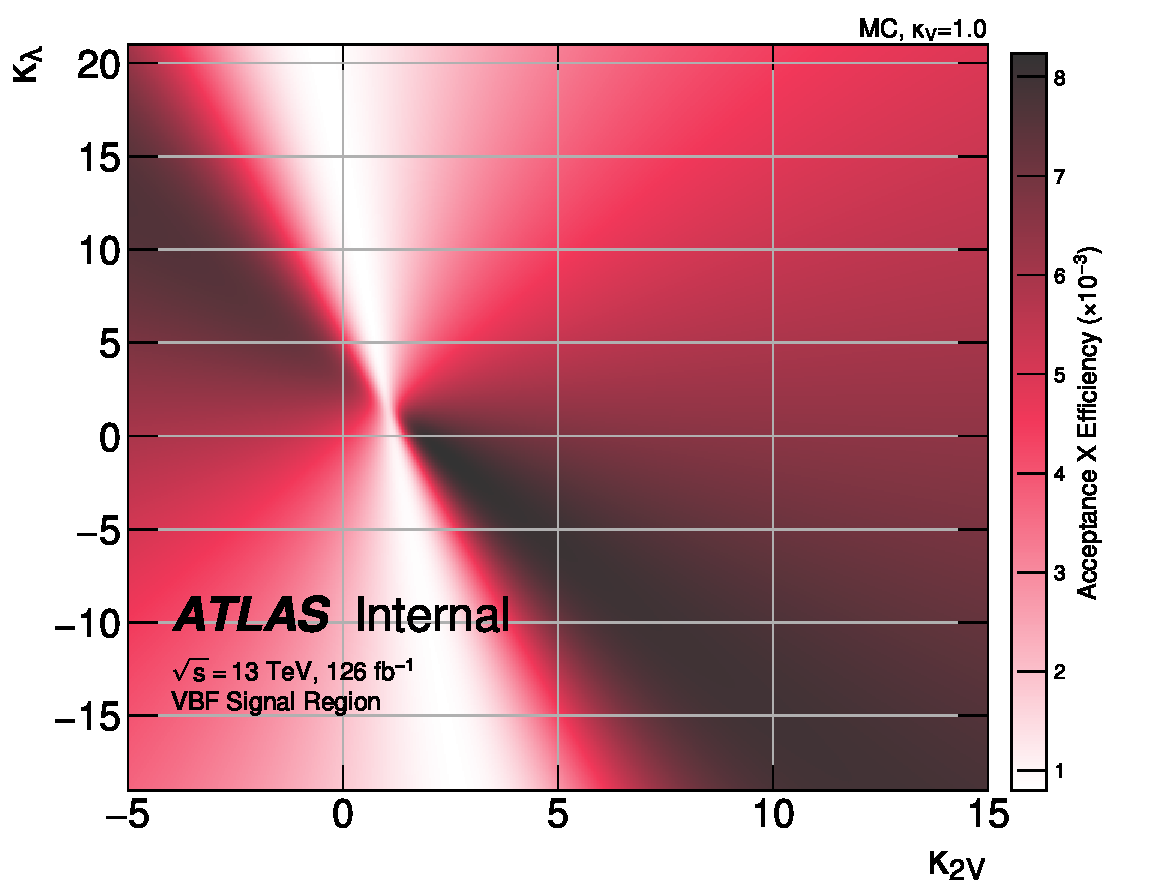
\includegraphics[width=\linewidth,height=\textheight,keepaspectratio]{selection/VBF2D-vbf-MC-Signal-Region-all-4b-accXeff-kv1p0}
                \caption{}
            \end{subfigure}\\
            \begin{subfigure}{0.48\textwidth}
                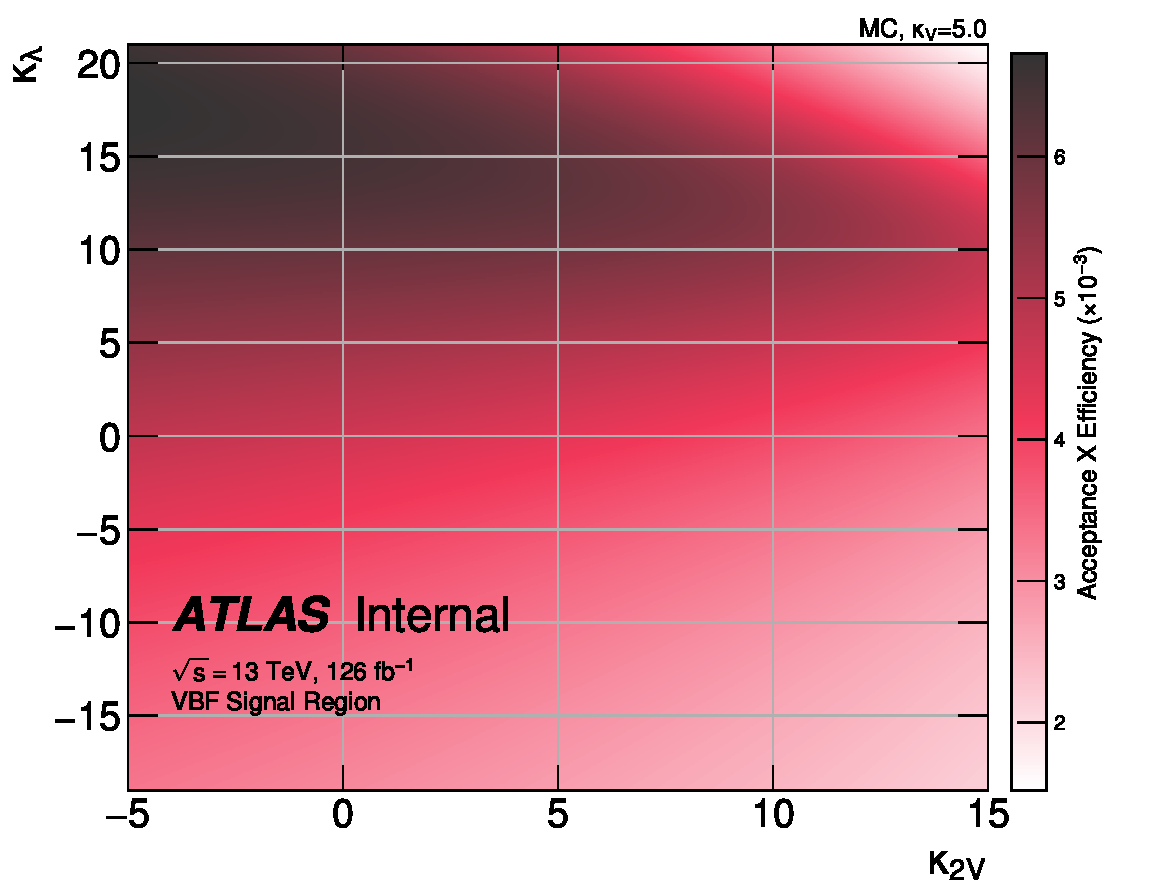
\includegraphics[width=\linewidth,height=\textheight,keepaspectratio]{selection/VBF2D-vbf-MC-Signal-Region-all-4b-accXeff-kv5p0}
                \caption{}
            \end{subfigure}
            \caption{
                Acceptance $\times$ Efficiency across the \kvv/\kl space for multiple values of \kv.
                These figures (and those that follow) indicate what fraction of signal events are expected (based on MC studies)
                    to both pass through ATLAS such that they are reconstructed (acceptance)
                    and subsequently remain after the various steps of selection (efficiency).
                Although the reconstruction and selection process is overall very punishing -- 
                    leaving roughly only one in every thousand signal events --
                    no particular variations of the signal model (i.e.\ no specific inputs of the $\kappa$ values)
                    are dramatically favored over any others;
                    all values visible across these plots lie within the same order of magnitude.
                The differences that do exist are result from varying the kappa values, which in turn alters the kinematics of the \vbfhhproc events.
                Different kinematic features can permit events to more easily pass reconstruction and selection.
            }
            \label{fig:accXeff_kv}
        \end{figure}

        \begin{figure}[tbh]
            \begin{subfigure}{0.48\textwidth}
                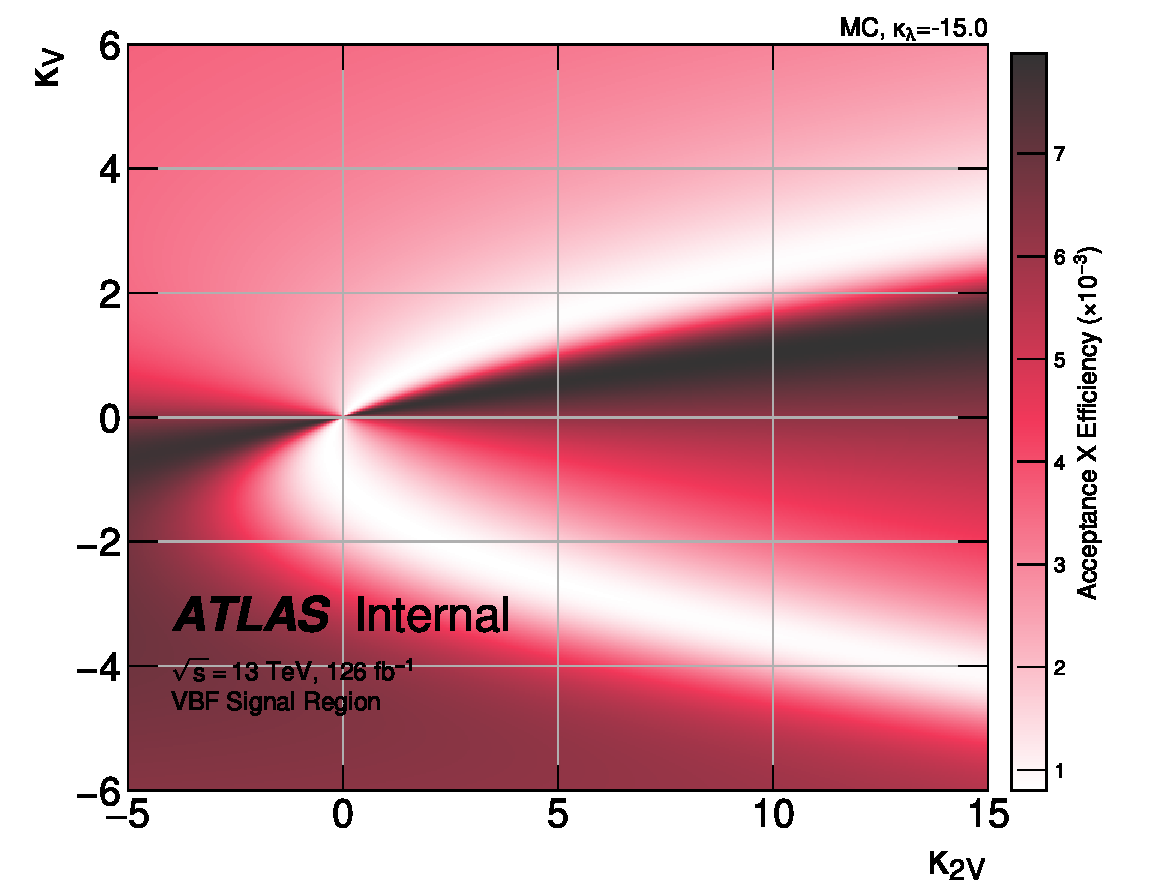
\includegraphics[width=\linewidth,height=\textheight,keepaspectratio]{selection/VBF2D-vbf-MC-Signal-Region-all-4b-accXeff-kl-15p0}
                \caption{}
            \end{subfigure}
            \begin{subfigure}{0.48\textwidth}
                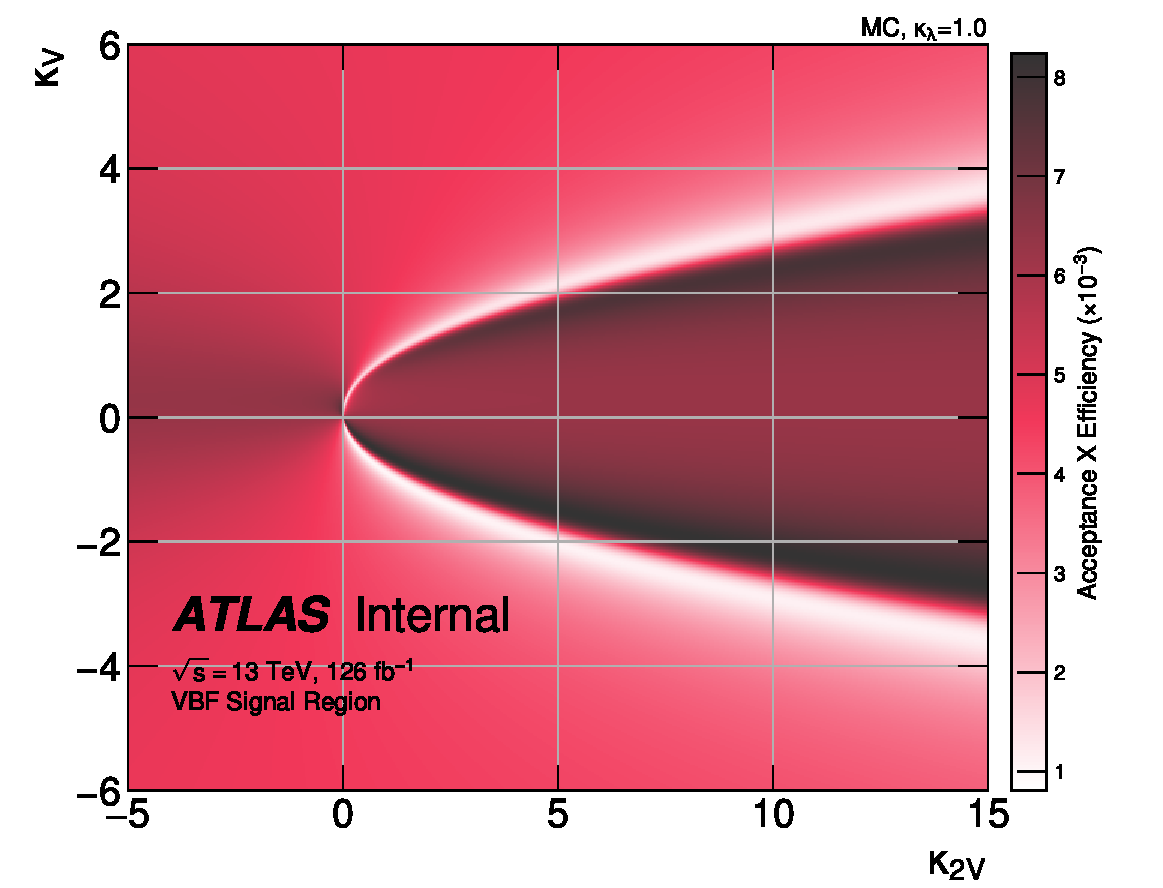
\includegraphics[width=\linewidth,height=\textheight,keepaspectratio]{selection/VBF2D-vbf-MC-Signal-Region-all-4b-accXeff-kl1p0}
                \caption{}
            \end{subfigure}\\
            \begin{subfigure}{0.48\textwidth}
                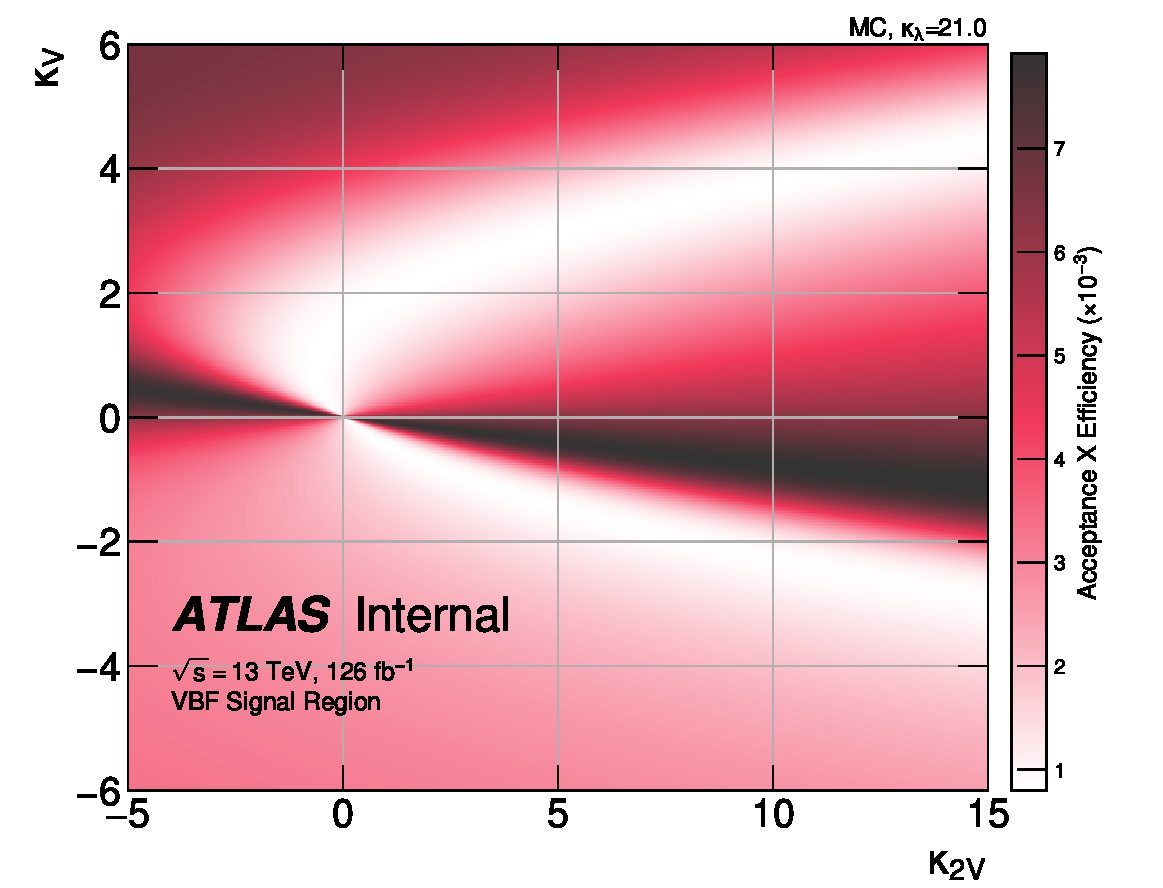
\includegraphics[width=\linewidth,height=\textheight,keepaspectratio]{selection/VBF2D-vbf-MC-Signal-Region-all-4b-accXeff-kl21p0}
                \caption{}
            \end{subfigure}
            \caption{
                Acceptance $\times$ Efficiency across the \kvv/\kv space for multiple values of \kl.
            }
            \label{fig:accXeff_kl}
        \end{figure}

        \begin{figure}[tbh]
            \begin{subfigure}{0.48\textwidth}
                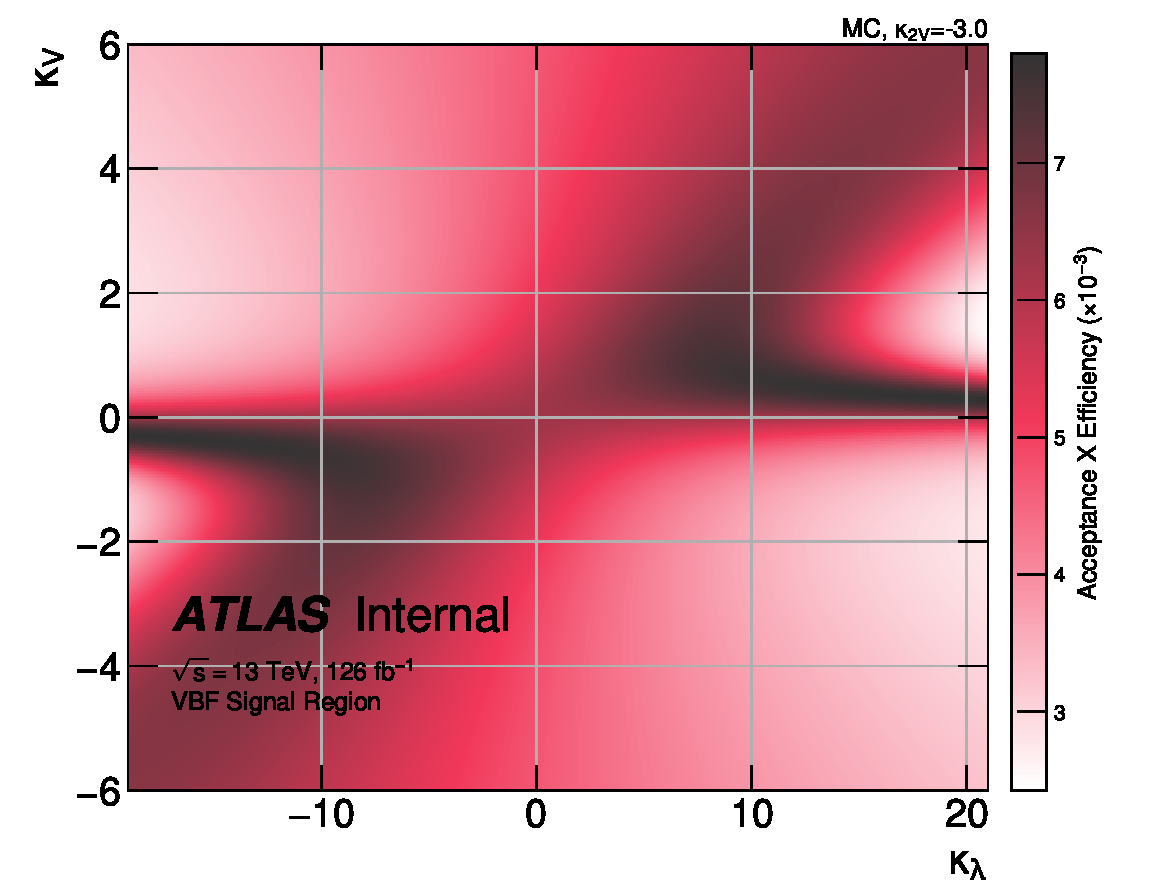
\includegraphics[width=\linewidth,height=\textheight,keepaspectratio]{selection/VBF2D-vbf-MC-Signal-Region-all-4b-accXeff-k2v-3p0}
                \caption{}
            \end{subfigure}
            \begin{subfigure}{0.48\textwidth}
                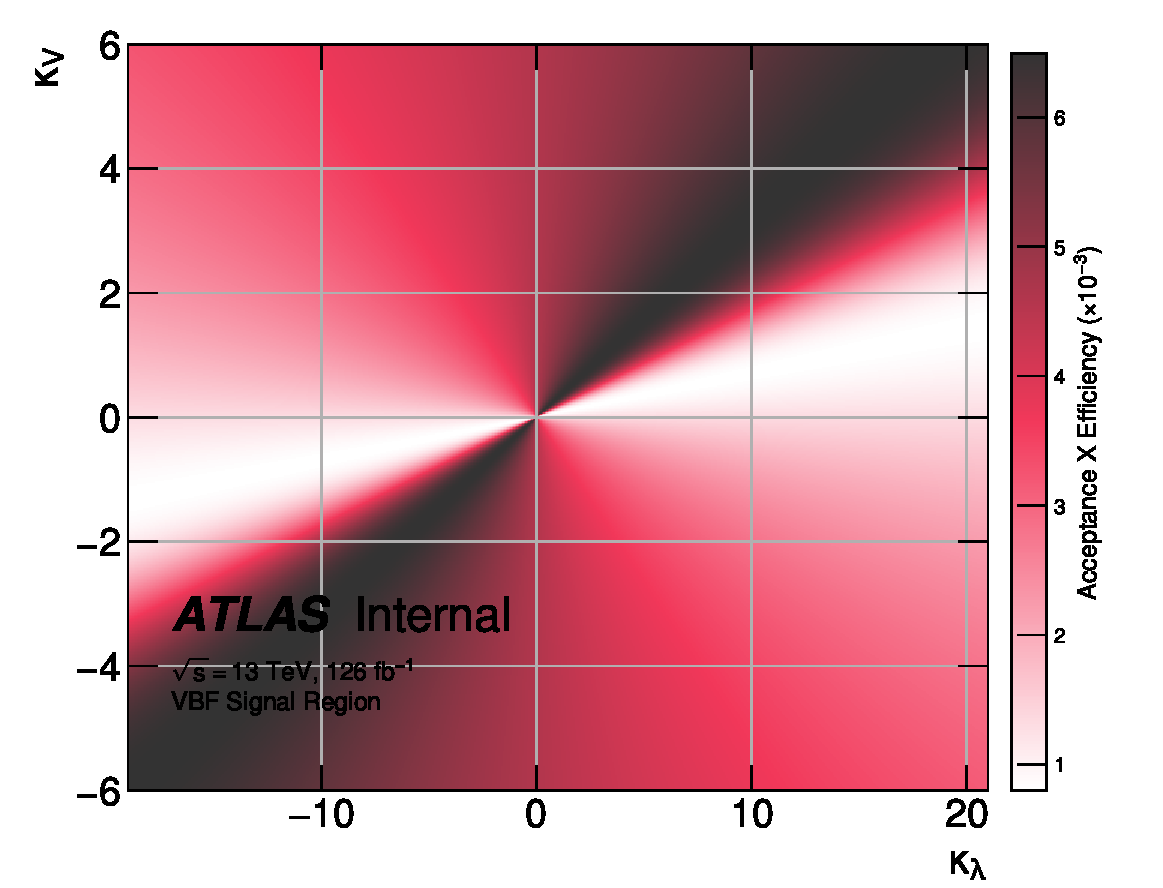
\includegraphics[width=\linewidth,height=\textheight,keepaspectratio]{selection/VBF2D-vbf-MC-Signal-Region-all-4b-accXeff-k2v0p0}
                \caption{}
            \end{subfigure}\\
            \begin{subfigure}{0.48\textwidth}
                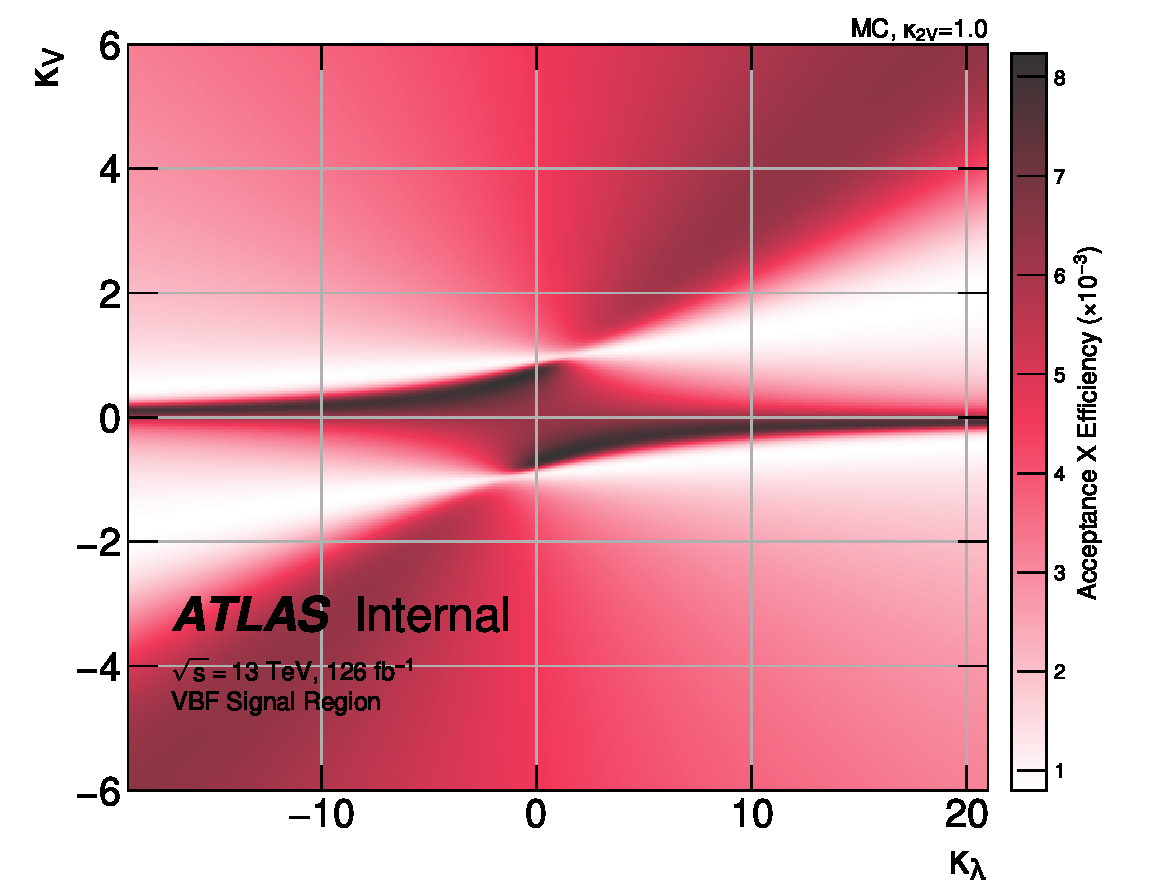
\includegraphics[width=\linewidth,height=\textheight,keepaspectratio]{selection/VBF2D-vbf-MC-Signal-Region-all-4b-accXeff-k2v1p0}
                \caption{}
            \end{subfigure}
            \begin{subfigure}{0.48\textwidth}
                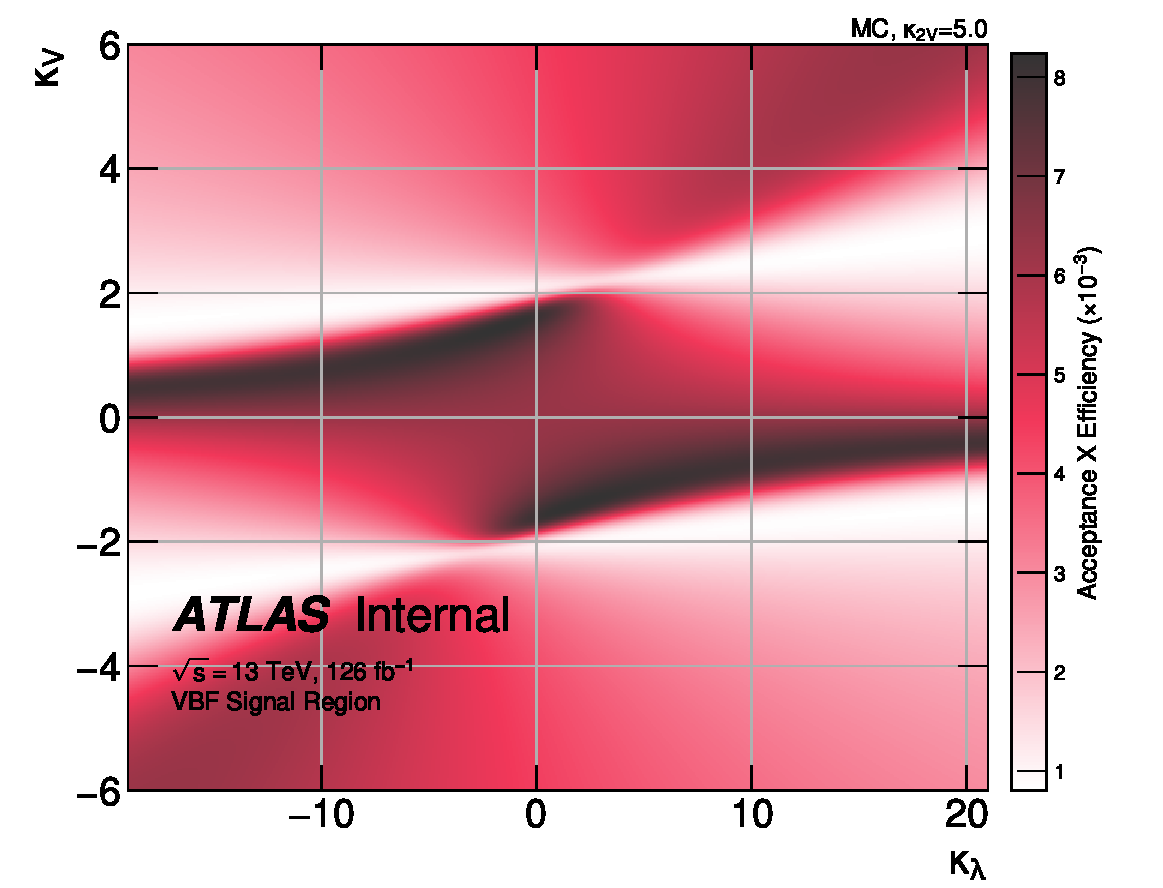
\includegraphics[width=\linewidth,height=\textheight,keepaspectratio]{selection/VBF2D-vbf-MC-Signal-Region-all-4b-accXeff-k2v5p0}
                \caption{}
            \end{subfigure}
            \caption{
                Acceptance $\times$ Efficiency across the \kl/\kv space for multiple values of \kvv.
            }
            \label{fig:accXeff_kvv}
        \end{figure}

            


